\chapter{مورد مطالعاتی}
در این فصل مطالعه‌ی موردی بر روی مجموعه‌داده‌ی \lr{defects4j} \cite{Just:2014:DDE:2610384.2628055} انجام می‌گیرد. ابتدا نحوه‌ی کلی برپایی آزمایش شرح داده می‌شود و سپس چگونگی استخراج معیارها و پیاده‌سازی ارمایش توضیح داده خواهد شد. 
\section{طراحی آزمایش}
به منظور ارزیابی رویکردهای گفته شده لازم است که برای مجموعه معیارهای هر رویکرد مدلهای پیش‌بینی ساخته شود و هر عملکرد هر مدل نسبت به پژوهش‌های گذشته مقایسه شود. به این ترتیب ابتدا لازم است از مجموعه‌داده‌ی فراهم شده معیارهای بیان شده در فصل \ref{sec:method} استخراج شوند. مجموعه‌داده‌ی \lr{defects4j} که در قسمت‌های آتی معرفی می‌شود شامل اطلاعات خطا در چندین فایل است و به همین تعداد، فایل بدون خطا در ثبت و پروژه‌ی متناظر به طور تصادفی انتخاب می‌گردد. برای فایلهای حاوی خطا و سالم، معیارها استخراج می‌شود. معیارهای استخراج شده  برای هر فایل به عنوان بردار ویژگی در مدلهای دسته‌بندی عمل می‌کند. مدلهای دسته‌بندی به منظور پیش‌بینی حاوی خطا بودن ساخته می‌شود و عملکرد آنها مقایسه می‌گردد. مدلهایی که با هم مقایسه می‌شود در الگوریتم و \واژه{پیکربندی} یکسان هستند و تنها تفاوت آنها در معیارهای استفاده شده به منظور یادگیری است. بدین ترتیب تاثیر معیارها بر پیش‌بینی خطا سنجیده می‌شود. 

\section{ آشنایی با ابزارها و مجموعه داده}
این قسمت به معرفی ابزارهای استفاده شده در این پژوهش می‌پردازد. آشنایی با این ابزارها به درک هرچه بهتر  نحوه‌ی استخراج معیارها  و روند آزمایش کمک می‌کند.

\subsection{مجموعه داده \lr{defect4j}}
 مجموعه‌‌داده‌ی انتخابی به منظور انجام مورد مطالعاتی لازم است که دارای ویژگی‌های زیر باشد:
 \begin{itemize}
 	\item
 	اطلاعات خطاهای پروژه وجود داشته باشد و این اطلاعات نشان دهد که خطا متعلق به کدام فایل در کدام ثبت است. 
 	\item
 	پروژه‌ها متن-باز باشد تا بتوان با استفاده از کد منبع آنها معیارها را استخراج نمود.
 	\item
 	برای پروژه‌ها موارد آزمون مناسب وجود داشته باشد تا بتوان معیارهای جهش را استخراج کرد.
 \end{itemize}
 در میان مجموعه‌داده‌های موجود مجموعه‌داده‌ی \lr{defects4j} تنها موردی است که تمام ویژگی‌ها را دارد.\\
 
این مجموعه شامل  شش پروژه می‌باشد که پنج مورد از آن‌ها مربوط به شرکت \نام{آپاچی}{Apache} است و دیگری نرم‌افزار jfreechart است که به شرکت خاصی تعلق ندارد. این پروژه‌ها  \واژه{متن-باز} هستند و با استفاده از نرم‌افزارهای کنترل نسخه‌ی گیت و svn می‌توان به کدهای آن‌ها در طول فرآیند توسعه‌ی آنها دسترسی پیدا کرد.
مجموعه‌داده‌ی \چر{defect4j} به صورت یک \واژه{چهارچوب} ارائه شده است که کارهایی بیش از نگهداری اطلاعات درباره‌ی پروژه‌ها انجام می‌دهد. مهم‌ترین  کارهایی که می‌توان به وسیله‌ی این ابزار انجام داده عبارت است در جدول زیر آمده است. 


\begin{table}[H] 
	\renewcommand*{\arraystretch}{1.3}	
	\centering \caption{عملیات‌های موجود در \چر{defects4j}  }
	\label{tab:defects4j-ops}
	\newcolumntype{C}{>{\centering\arraybackslash} m } 
	\begin{tabular}{ |c|c|}
		
		\hline
		\hline
		نام عملیات  & توضیح
		\\
		\hline
		\hline
		\lr{info } &   نمایش پیکربندی یک پروژه‌ی خاص یا خلاصه‌ی یک خطای خاص
		\\
		\hline
		\lr{checkout} &   وارسی یک نسخه‌ی حاوی خطا یا تعمیر شده از پروژه
		\\
		\hline
		\lr{compile} &   کامپایل کدهای و آزمون‌های نوشته شده توسط توسعه‌دهندگان
		\\
		\hline
		\lr{test} &   اجرای یک آزمون یا مجموعه‌ی آزمون در یک نسخه‌ی حاوی خطا یا تعمیر شده از پروژه
		\\
		\hline
		\lr{mutation} &   اجرای تحلیل جهش در یک نسخه‌ی حاوی خطا یا تعمیر شده از پروژه
		\\
		\hline
		
	\end{tabular}
\end{table}

این ابزار در اجرای عملیات‌های بالا دارای محدودیت است و تنها آن‌ها را بر روی ثبت‌های از پیش تعیین شده انجام می‌دهد. ثبت‌های از پیش تعیین شده شامل ثبت‌های حاوی خطا و تعمیر آن خطا می‌باشد. در جدول زیر اطلاعات مربوط به تعداد خطاهای هر پروژه آمده است. 

\begin{table}[H] 
	\renewcommand*{\arraystretch}{1.3}	
	\centering \caption{پروژه‌های موجود در \چر{defects4j}  }
	\label{tab:defects4j-bugs}
	\newcolumntype{C}{>{\centering\arraybackslash} m } 
	\begin{tabular}{ |c|c|c|}
		
		\hline
		\hline
	نام مختصر &	نام کامل  & تعداد خطا
		\\
		\hline
		\hline
		\lr{Chart } & JFreeChart &	26
		\\
		\hline
		\lr{Closure} & \lr{Closure compiler}	& 133
		\\
		\hline
		\lr{Lang} &   \lr{Apache commons-lang} &	65
		\\
		\hline
		\lr{Math} &  \lr{Apache commons-math} &	106
		\\
		\hline
		\lr{Mockito} &   Mockito &	38
		\\
		\hline
		Time & Joda-Time &	27
		\\
		\hline
		
	\end{tabular}
\end{table}


به منظور نصب و راه اندازی این ابزار ابتدا از صفحه ی github آن پروژه بر روی  PC ، کلون می شود. سپس یک script باید اجرا کرد تا سایر تعلقات پروژه دانلود شود. این تعلقات شامل مخزن نرم افزاری مربوط به این این شش پروژه است که کدهای پروژه ها در آن قرار دارد. نکته ی قابل توجه در این پروژه این است بجز  دستور info سایر دستورات عملیاتهای مربوط را بر روی کامپیوتر کاربر انجام می‌دهند و خروجی را نمایش می‌دهند نه اینکه از یک پایگاه داده اطلاعات صرفاً بارخوانی شوند. 
در نیازمندی های این ابزار اشاره شده که باید از جاوا نسخه ی ۷ استفاده شود. اما مسأله ای که به آن اشاره نشده توزیع کننده ی جاوا است. جاوا دو توزیع کننده ی عمده دارد. یکی OpenJDK و دیگر Oracle. در ابتدا از نسخه ی openJDK استفاده شد زیرا نصب آن در linux ساده‌تر است و همچنین oracle به ایرانیان اجازه ی دانلود نمی دهد. اما با openJDK ابزار defects4j و ابزارهایی که به آن وابسته است به خوبی کار نمی کنند. به عنوان مثال برخی مجموعه تست ها که باید بدون خطا اجرا شوند به دلیل نبود dependency های لازم با شکست مواجه می شوند. این مسأله موجب سردرگمی و صرف مدت زمانی تا حل آن شد. 
راه ارتباط با این ابزار command line‌ می‌باشد و نمونه‌ ای از دستورات قابل استفاده در این ابزار  در شکل  \ref{fig:d4j-info-command} است که این دستور اطلاعات مربوط به پروژه ی Lang خطای شماره ی یک را خواهد داد. 
\begin{latin}
	\flushleft
defects4j info -p Lang -b 1
\end{latin}

\begin{figure}[H]
	\centering
	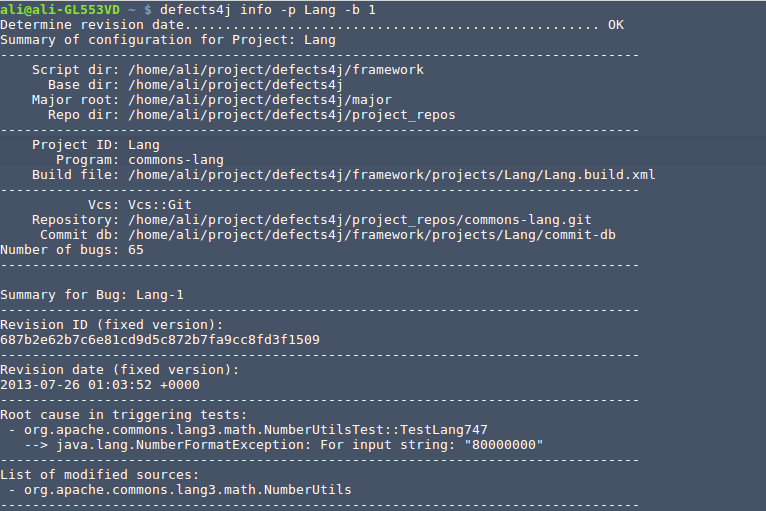
\includegraphics[width=.8\textwidth]{img/case_study/d4j-info-commadn.png}
	\caption{اجرای دستور info در \lr{defects4j}}
	\label{fig:d4j-info-command}
\end{figure}

\subsection{ابزار Major}

این ابزار جهت تولید جهش یافته و تحلیل جهش استفاده می شود. در ابتدا تصمیم بر این بود از ابزار دیگری به نام PIT استفاده شود ولی ابزارdefect4j از major استفاده می‌کند بنابرین به دلیل سازگاری با D4j و نیز قابلیت‌های منحصر به فرد این ابزار تصمیم به استفاده از Major  گرفته شد. چند مورد از ویژگی‌ها عبارتند از :
\begin{itemize}

\item
 راحتی استفاده: قابلیت تعامل از روشهای مختلف مانندcommand lineِ، بکارگیری به وسیله ی ابزار build ant و دستورات کم نسبت به PIT
\item
 مجموعه عملگرهای کاملتر
\item
 راحتی در پیکر بندی : امکان انجام تحلیل تنها برای یک کلاس یا تابع، تنظیمات راحت و کامل جهت مشخص کردن مجموعه عملگرها
\end{itemize}
لازم به ذکر است که این ابزار از compiler‌ مخصوص به خود جهت کامپایل برنامه و ساخت جهش یافته استفاده می‌کند که گسترش یافته ی یک کامپایلر جاوا است. 
البته در انتها مشخص شد که این برنامه کاستی هایی هم دارد از جمله کامل نبود مستندات برای بکارگیری پیشرفته و خطاهایی که در قسمت مربوطه به آن‌ها اشاره خواهد شد. 
استفاده از این ابزار را می‌توان در سه مرحله خلاصه کرد :
\begin{enumerate}
\item

پیکربندی تولید جهش یافته به وسیله MML script: این ابزار برای مشخص نمودن اینکه از چه عملگرهای استفاده شود و آن‌ها در چه محل هایی از برنامه به کار گرفته شوند یک زبان ساده ابداع کرده است به نام MML که یک کامپایلر نیز دارد. ابتدا کد mml نوشته می‌شود سپس با mmlc کامپایل می‌شود و نتیجه به عنوان یکی از پارامترها به در هنگام فراخوانی ابزار ارسال می شود. نمونه‌ای از این کد در شکل \ref{fig:major-mml} آمده است. 

\begin{figure}[H]
	\centering
	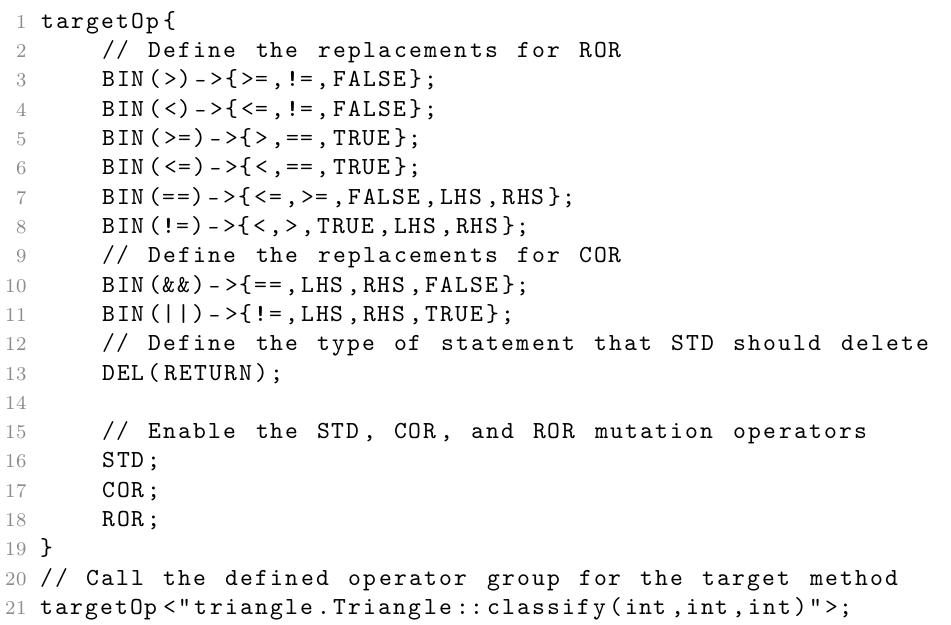
\includegraphics[width=.8\textwidth]{img/case_study/major-mml.png}
	\caption{نمونه کد MML در Major}
	\label{fig:major-mml}
\end{figure}
\item 	
تولید جهش یافته ها: برای این منظور می‌توان از command line یا فایل build.xml مربوط به پروژه استفاده کرد که روش دوم مورد استفاده قرار گرفت. برای این منظور لازم است که یک قطعه کد به شکل زیر به فایل build.xml اضافه شود. و سپس برنامه کامپایل شود. حاصل به شکل زیر خواهد بود که نشان می‌دهد ۸۶ جهش یافته تولید شده است. همچینین ابزار یک فایل به نام mutation.log تولید می‌کند که نشان می‌دهد چه جهش یافته هایی در کجا تولید شده اند. 

\begin{figure}[H]
	\centering
	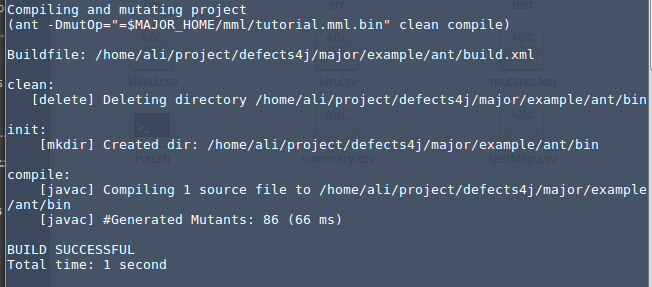
\includegraphics[width=.8\textwidth]{img/case_study/major-mutant.png}
	\caption{نمونه کد MML در Major}
	\label{fig:major-mutant}
\end{figure}

\begin{figure}[H]
	\centering
	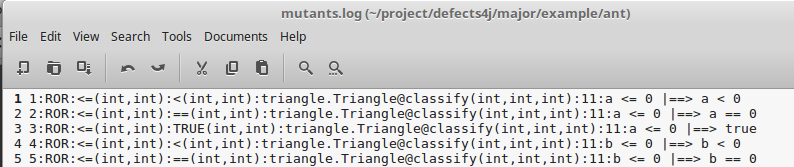
\includegraphics[width=.8\textwidth]{img/case_study/major-log.png}
	\caption{نمونه کد MML در Major}
	\label{fig:major-log}
\end{figure}

\item
 اجرای تحلیل جهش : در این قسمت نیز قطعه کدی به فایل build.xml اضافه می‌شود و سپس فایل اجرا می شود. در اجرا ابتدا فایل‌های تست کامپایل می‌شود و سپس هر مجموعه تست بر روی جهش یافته هایی که تا کنون کشته نشده‌اند اجرا می شود. در پایان نتایج را در خروجی چاپ می کند. همچنین نتایج را در فایلهای با پسوند csv قرار می دهد. نمونه‌ای از اجرای تحلیل جهش و فایلهای خروجی در زیر آمده است:
 
 \begin{figure}[H]
 	\centering
 	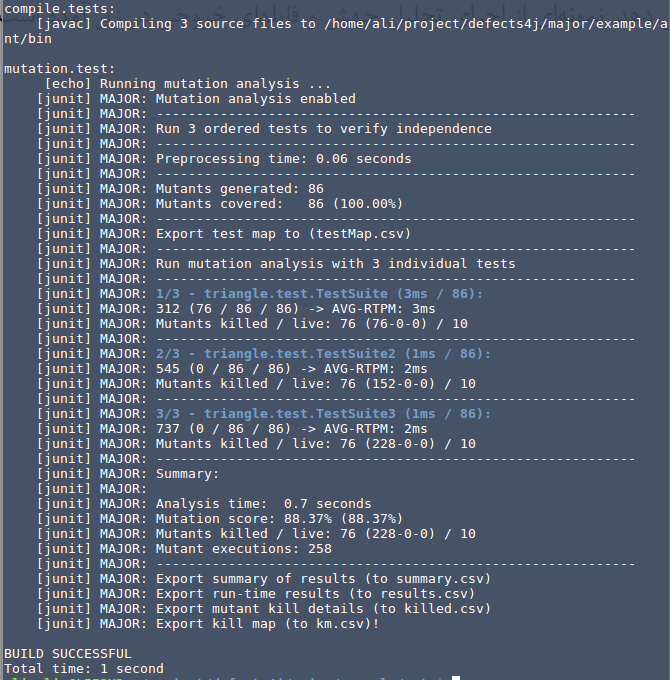
\includegraphics[width=.8\textwidth]{img/case_study/major-analysis.png}
 	\caption{نمونه کد MML در Major}
 	\label{fig:major-analysis}
 \end{figure}
 
 \begin{figure}[H]
 	\centering
 	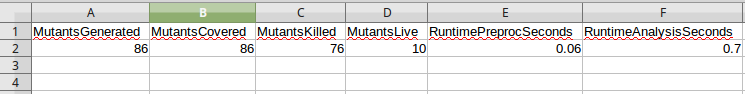
\includegraphics[width=.8\textwidth]{img/case_study/major-results.png}
 	\caption{نمونه کد MML در Major}
 	\label{fig:major-results}
 \end{figure}

\end{enumerate}


\subsection{کتابخانه‌ی Jgit}
این کتابخانه جهت کار با مخازن نرم افزاری از نوع git به کار گرفته می‌شود و به زبان جاوا است. تمام عملیات های مهم و اساسی که در نرم‌افزار اصلی git وجود دارد در این کتابخانه نیز قابل انجام است. مشکلی که کار با این کتابخانه دارد نبود منابع آموزشی به اندازه ی کافی است. چراکه کاربران زیادی ندارد و آموزش‌های ابتدایی معمولاً نیازهایشان را بر طرف می کند. 
\subsection{چهارچوب Hibernate }
به وسیله ی این چارچوب می‌توان  اشیاء موجود در برنامه ی جاوا را به داده‌های موجود در پایگاه داده تبدیل کرد. اصطلاحاً به این ابزار ها ORM (object relational mapping)  می گویند. در ابتدا تصمیم بر این بود که داده‌های بدست آمده در فایل متنی ذخیره شوند و در هنگام نیاز آن‌ها خوانده شوند یا همه ی اشیاء با هر بار اجرا ساخته شوند نکات زیر سبب شد که هزینه ی اول کار با پایگاه داده و مزایای بلند مدت آن به سادگی استفاده از فایل متنی ترجیح داده شود:
۱- هر بار ساخت اشیاء با اجرای برنامه بسیار زمانبر است و اتلاف وقت زیادی دارد
۲- لازم است برای اطمینان از درستی برنامه، داده‌ها در قالب جداولی به صورت چشمی کنترل شوند
۳- فراخوانی و جستجو در پایگاه داده سریع است و کارایی بالا می‌رود
۴- نگهداری از برنامه در دراز مدت راحت‌تر خواهد بود و خوانایی کدها بیشتر خواهد بود چرا که کار با پایگاه داده دارای اصول مشخصی است و سایرین از آن اطلاع دارند اما فایل متنی اینگونه نیست

\section{نکات پیاده‌سازی پروژه}

پیاده‌سازی پروژه در زبان جاوا انجام گرفت. یکی از نکات مهم و قابل توجه در پیاده‌سازی این پروژه این است که تمام مراحل انجام کار  به طور کاملاً خودکار انجام شود و در هیچ مرحله‌ای نیاز به دخالت عامل خارجی  ندارد بجز پیکربندی اولیه مانند آدرس پایگاه داده. همچنین در تمام مراحل سعی شده است که تمام اصول لازم در طراحی معماری نرم‌افزار به کار گرفته شود و نیازمندی‌های کیفی پروژه نیز مد نظر قرار گیرد. این نیازمندی‌ها شامل موارد زیر است:
\begin{enumerate}
\item 
\واژه{کارایی} : جهت پاسخ به این نیازمندی از پایگاه داده استفاده شده است.
\item
قابلیت نگهداری: این قابلیت از سایرین بیشتر حائز اهمیت است. زیرا پروژه های پروژهشی خود به صورت مستقیم کاربران عمومی ندارند و از این جهت نیازمند کارایی بالا یا رابط گرافیکی کاربر پسند نیستند. استفاده آن‌ها معمولاً در گسترش آن‌ها توسط سایر محققین است که راه را ادامه خواهند داد. 
\begin{itemize}
\item

 برای پاسخ به این نیازمندی اصول مربوط به کدنویسی  در فصل سوم و چهارم کتاب  \cite{martin2009clean} به کار گرفته شده است.
 \item
 از الگوهای نرم افزاری پر کاربرد مانند \نام{اداپتور}{Adaptor}،  \نام{فکتوری}{Factory} و \نام{سینگلتون}{Singelton} استفاده شده است.
 \item
 به منظور جلوگیری از قطعه کد تکراری از وراثت و توابع \واژه{عمومی} استفاده شده است. همینطور عمق وراثت از عدد ۳ بیشتر نشده است زیرا وراثت عمیق از خوانایی کد می‌کاهد و محل اشتباه خواهد بود. 
\end{itemize}
\item
امنیت: از آنجا که پروژه قرار نیست به استفاده ی عموم برسد و کاربران عمل متخاصمانه‌ای انجام نخواهند داد   به نوع خاصی از امنیت  نسبت به انواع متداول دارد.  باید روند توسعه‌ی پروژه دارای امنیت باشد. از این نظر که کدها مفقود نشوند یا در صورت اشتباه در توسعه بتوان پروژه را به حالت قبل بازگرداند. در این راستا کدهای پروژه در مخزن نرم افزاری از نوع گیت نگهداری شده که یک مخزن در کامپیوتر شخصی و دیگری در سایت \نام{بیت‌باکت}{Bitbucket - \url{https://bitbucket.org/alimohebbi/bug_predict }} 
قرار دارد. مزیت این سایت نسبت به گیت‌هاب این است مخازن خصوصی  را به صورت رایگان ارائه می دهد. در مخازن خصوصی  اجازه‌ی دسترسی تنها به  افراد تعیین شده از طرف مالک  داده می‌شود و عموم کاربران به آن دسترسی ندارند. از ابتدای شروع پیاده‌سازی کدها در مخازن بروزرسانی شده است. نمایی از ثبت‌های مختلف پروژه در مخزن در شکل \ref{fig:bitbucket}
آورده شده است. 
\end{enumerate}

 \begin{figure}[H]
	\centering
	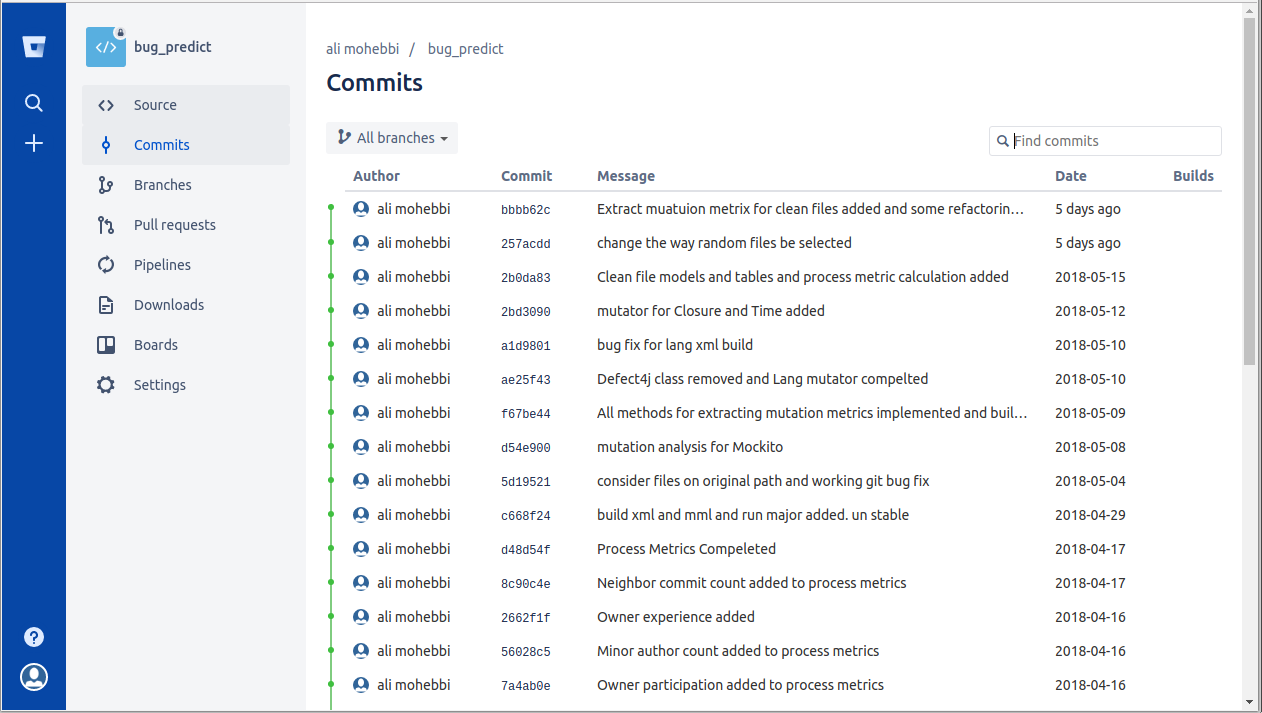
\includegraphics[width=1\textwidth]{img/case_study/bitbucket.png}
	\caption{نمایی از مخزن نرم‌افزاری}
	\label{fig:bitbucket}
\end{figure}



\section{رویکرد اول : معیارهای فرآیند در کنار جهش}
در این قسمت  چگونگی استخراج معیارهای رویکرد اول شرح داده می‌شود. ابتدا لازم است اطلاعات مربوط به ثبت‌های  حاوی خطا از ابزار \lr{defects4j} بازیابی شود و سپس این اطلاعات با استفاده از مخرن نرم‌افزاری تکمیل شود. در مراحل بعد ابتدا معیار‌های فرآیند و سپس معیارهای جهش استخراج خواهند شد. 

\subsection{ استخراج اطلاعات مربوط به ثبت‌های   حاوی خطا}
اطلاعاتی که درباره‌ی ثبت‌های حاوی خطا قابل بازیابی است در زیر آمده است:
\begin{enumerate}
\item شناسه‌ی ثبت در مخزن 
\item نام فایل حاوی خطا
\item شماره ی خطا در ابزار \lr{defects4j}
\item شماره‌ی ثبت تعمیر خطا
\item نام پروژه
\item نام انتشار قبلی پروژه
\item شماره‌ی ثبت انتشار قبلی پروژه
\end{enumerate}

از میان اطلاعات بالا همگی به سادگی با استفاده از ابزار defect4j قابل استخراج است بجز دو مورد آخر. همچنین شماره‌ی ثبت تعمیر مورد استفاده قرار نگرفت ولی نگهداری شد چراکه ممکن بود لازم شود. 
برای بدست آوردن اطلاعات مربوط به هر انتشار لازم است که مخرن نرم افزاری هر پروژه مورد بررسی قرار گیرد. در  مخازن پروژه‌های نرم‌افزاری  از نوع گیت برای مشخص کردن یک رویداد مهم از \نام{تگ}{Tag} استفاده می‌شود. هر تگ می‌تواند به یک ثبت از برنامه اشاره کند. تگ می‌تواند نمایانگر رویدادهایی چون انتشار برنامه، انتشار بتا، و یا کاندید انتشار باشد. بنابرین با استفاده از تگ می‌تواند انتشار را پیدا کرد.\\

تگ‌های مخازن گیت دو نوع \واژه{سبک‌وزن} و \واژه{حاشیه‌نویسی شده} که در میان پروژه‌های مورد مطالعه از هر دو نوع جهت مشخص کردن انتشار استفاده شده است.  کار کردن با این دو نوع تگ دارای تفاوتهایی در پیاده‌سازی است که در ایتجا از پرداختن به جزییات صرف نظر می‌شود. \\ ابتدا همه‌ی تگ‌های موجود در مخازن نرم‌افزاری استخراج می‌شود و در پایگاه داده قرار می‌گیرد. از میان تگ‌های استخراج شده تگ‌های نا مرتبط با انتشار از پایگاه داده حذف می‌شود. تگ‌های نامرتبط با توجه به نام آنها مشخص می‌شود به عنوان مثال تگ‌هایی که حاوی لغات Beta یا Dev هستند نامرتبط  محسوب می‌شوند. در نهایت جدولی به نام ReleaseProject ساخته می‌شود که در آن اطلاعات انتشارهای مختلف وجود دارد. نمایی از این جدول در شکل \ref{fig:project-release} آمده است. \\
\begin{figure}[H]
	\centering
	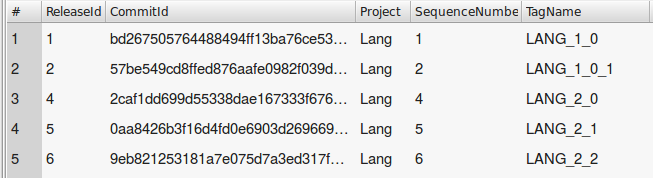
\includegraphics[width=1\textwidth]{img/case_study/project-release.png}
	\caption{نمایی از جدول محتوای انتشارها}
	\label{fig:project-release}
\end{figure}


در قدم بعدی باید مشخص شود اولین انتشار ما قبل هر ثبت حاوی خطا کدام است. برای این منظور لیست ثبت‌ها  در یک پروژه به ترتیب زمانی بررسی می‌شود. اولین ثبت  ماقبل ثبت مورد نظر که مربوط به یک انتشار است یافت می‌شود و به عنوان انتشار ماقبل آن ثبت در نظر گرفته می‌شود. \\

 در نهایت جدولی به نام BugInfo تولید شده که نمایی از آن در شکل \ref{fig:bug-info} آمده است. این جدول ۴۰۵ سطر دارد که بیشتر از تعداد کل خطاهای ذکر شده در مجموعه داده‌ی \lr{defects4j} است. علت این است که یک خطا می‌تواند خطا در چندین پرونده به طور همزمان باشد و از آنجا که پیش‌بینی در سطح پرونده انجام می‌شود لازم است اطلاعات برای پرونده‌ها ذخیره شود.

\begin{figure}[H]
\centering
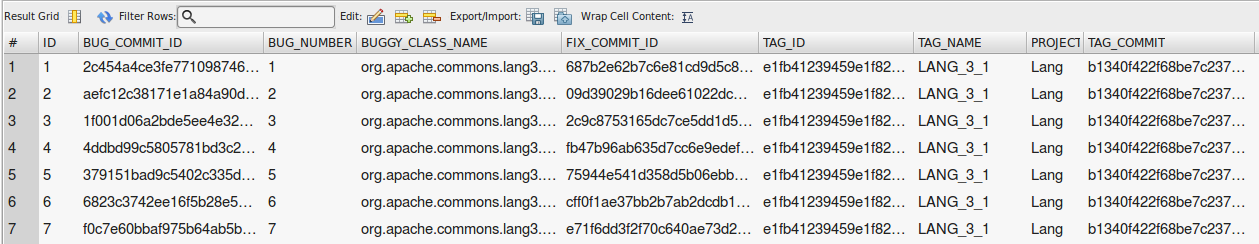
\includegraphics[width=1\textwidth]{img/case_study/bug-info.png}
\caption{نمایی از جدول محتوای اطلاعات پرونده‌های حاوی خطا}
\label{fig:bug-info}
\end{figure}

\subsection{انتخاب پرونده‌های سالم}
همانطور که مطرح شد تعداد پرونده‌های حاوی خطا برابر ۴۰۵ عدد است که از تعداد کل پرونده‌ها کمتر است. بنابرین جهت ساخت مدلهای بدون جهت‌گیری به همین تعداد پرونده‌های بدون خطا به طور تصادفی انتخاب می‌شود. بدین ترتیب یک مجموعه داده‌ی \واژه{متعادل} حاوی ۸۱۰ پرونده ساخته شده است. این روش طبق مقاله‌ی \cite{johannessen2008data} به کار گرفته شده است. در این انتخاب به تعداد پرونده‌های حاوی خطا، پرونده‌های بدون خطا انتخاب می شود. \\به ازای هر پرونده‌ی دارای خطا در همان ثبت از پروژه‌ی مربوط یک پرونده‌ی بدون خطا به صورت تصادفی انتخاب می‌شود. برای این کار لیست تمام پرونده‌های داخل پروژه در ثبت فایل حاوی خطا در نظر گرفته می‌شود و یک فایل به صورت تصادفی انتخاب می‌شود. این پرونده نباید جز پرونده‌های حاوی خطا در آن ثبت از  پروژه باشد.  البته ممکن اسن پرونده در ثبت‌های بعدی یا قبلی خطا داشته باشد و از این نظر محدودیتی ندارد. همانطور که گفته شد یک ثبت ممکن از بیش از یک فایل حاوی خطا داشته باشد. سپس مشخصات این فایل در جدول CleanInfo قرار می گیرد. نمایی از این جدول در تصویر \ref{fig:clean-info} آورده شده است.
\begin{figure}[H]
	\centering
	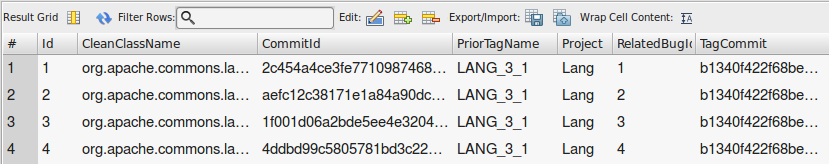
\includegraphics[width=1\textwidth]{img/case_study/clean-info.png}
	\caption{نمایی از جدول محتوای اطلاعات پرونده‌های سالم}
	\label{fig:clean-info}
\end{figure}



\subsection{ استخراج معیارهای فرآیند}
در  این قسمت نحوه‌ی استخراج هر یک از معیارهای ذکر شده در قسمت \ref{sec:method-phase1} بیان می‌شود. \\
\textbf{‫تعداد ثبت در سیستم کنترل نسخه‬:}
اولین راه حلی که به ذهن می‌رسد استفاده ی مستقیم از Jgit برای این کار است.  به این صورت که تعداد ثبت‌های بین ثبت کنونی و انتشار قبلی  بررسی کرده و تعداد  ثبت‌هایی که در آن‌ها فایل حاوی خطا تغییر کرده است شمرده شوند. مشکل این راه این است که بسیار پر هزینه  خواهد بود زیرا مرتبا باید عملیات \واژه{ورودی/خروجی} بر روی دیسک انجام پذیرد و همچنین بررسی‌های تکراری بسیاری انجام می‌گیرد. به عنوان مثال دو ثبت حاوی خطا را در نظر بگیرید که دارای انتشار ما قبل یکسانی هستند. تعدادی از بررسی‌های ثبت‌های ما بین آن‌ها تا ثبت مربوط به انتشار دارای همپوشانی خواهد بود. از طرف دیگر می‌توان اطلاعاتی که در بررسی ثبت‌ها بدست می‌آید در محاسبه‌ی معیارهای دیگر نیز مورد استفاده قرار گیرد.\\

همچنین برای یافتن ثبت‌های بین انتشار و ثبت مورد نظر نمی‌توان از تاریخ ثبت آنها استفاده کرد. زیرا تعداد زیادی از ثبت‌های ابتدای  برخی پروژه ‌های مورد مطالعه دارای تاریخ یکسانی هستند استفاده از تاریخ غیر ممکن می‌شود. علت داشتن تاریخ یکسان احتمالاً مهاجرت از یک نوع مخرن نرم‌افزاری به نوع گیت بوده است. \\

 بنابرین کل ثبت‌های پروژه‌ها مورد بررسی قرار گرفت و دو جدول تولید شد.
جدول اول به نام CommitInfo‌ که اطلاعات کلی ثبت‌ها را در بر می‌گیرد و جدول دوم  CommitChangedFile که اطلاعات مربوط به پرونده‌هایی که در یک ثبت از برنامه نسبت به ثبت قبلی تغییر کرده است نگهداری می‌شود.  در این جدول برای هر پرونده تعداد خطوط اضافه و کم شده نسبت به ثبت قبلی ذخیره شده است. در جدول اول \lr{Sequence\textunderscore Number} نشان می‌دهد که چندمین نسخه از ابتدای پروژه می‌باشد و این عدد در هنگام بررسی‌ها به آن ثبت داده‌ شده زیرا برای یافتن ثبت‌های بین ثبت کنونی و ثبت مربوط به انتشار قبلی لازم است از آنها استفاده شود. \\
  هر سطر از جدول دوم یک کلید خارجی دارد به سطری از جدول اول. قسمتی از جدول CommitInfo  در شکل \ref{fig:commit-info} و جدول CommitChangeFile در شکل \ref{fig:change-file-info}  زیر آمده است:

\begin{figure}[H]
	\centering
	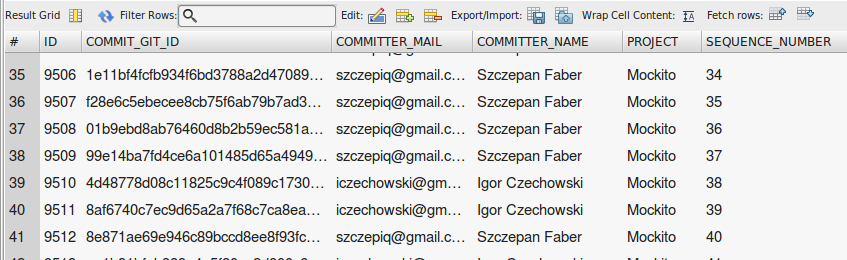
\includegraphics[width=1\textwidth]{img/case_study/commit-info.png}
	\caption{نمایی از جدول اطلاعات ثبت‌ها}
	\label{fig:commit-info}
\end{figure}


\begin{figure}[H]
	\centering
	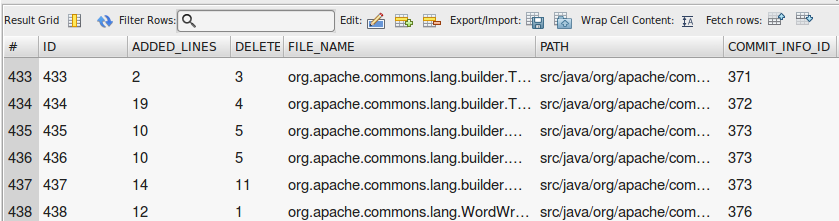
\includegraphics[width=1\textwidth]{img/case_study/change-file-info.png}
	\caption{ نمایی از جدول تغییرات پرونده‌ها در ثبت‌ها }
	\label{fig:change-file-info}
\end{figure}

در نهایت با استفاده از قطعه کد \ref{code:commit-info} اطلاعات مربوط به ثبت مورد نظر و ثبت انتشار بازیابی می‌شوند و سپس  از شماره‌ی دنباله‌ی آنها در پرسمان موجود در قطعه کد \ref{code:ncomm} استفاده می‌شود و معیار محاسبه می‌گردد.



\begin{latin}
	\begin{lstlisting}[language=SQL]
SELECT  * from CommitInfo CI where CI.COMMIT_GIT_ID = :gitId AND CI.PROJECT = :project
\end{lstlisting}
\end{latin}
\captionof{lstlisting}{بازیابی اطلاعات ثبت}
\label{code:commit-info}

\begin{latin}
\begin{lstlisting}[language=SQL]
SELECT  count(*) from CommitChangedFile CC where CC.COMMIT_INFO_ID IN
	(SELECT CI.ID from CommitInfo CI WHERE CI.SEQUENCE_NUMBER BETWEEN 
	 :startSeq AND :endSeq AND CI.PROJECT = :project)
AND CC.FILE_NAME = :fileName
\end{lstlisting}
\end{latin}
\captionof{lstlisting}{محاسبه‌ی معیار تعداد ثبت‌ در سیستم کنترل نسخه}
\label{code:comm}

\متن‌سیاه{‫تعداد توسعه‌دهندگان فعال:‬}
به منظور محاسبه‌ی این معیار تعداد آدرس ایمیل‌های ثبت‌کننده‌های ثبت‌هایی شمرده می‌شود که آن ثبت‌ها شماره‌ی دنباله‌ی آنها بین شماره‌ی دنباله‌ی ثبت پرونده‌ی مورد نظر و ثبت انتشار قبلی است و همچنین در آن ثبت پرونده‌ی مورد نظر در آن ثبت‌ها تغییر کرده است. به عبارت دیگر ثبت‌هایی که نام پرونده در جدول  CommitChangeFile  برای آن‌ها وجود دارد. 

\begin{latin}
\begin{lstlisting}[language=SQL]
SELECT  count(DISTINCT CI.COMMITTER_MAIL) from CommitInfo CI WHERE
CI.SEQUENCE_NUMBER BETWEEN :startSeq AND :endSeq AND CI.PROJECT = 
project AND CI.ID IN 
	(SELECT CC.COMMIT_INFO_ID from CommitChangedFile CC where CC.FILE_NAME = :fileName)
\end{lstlisting}
\end{latin}
\captionof{lstlisting}{محاسبه‌ی تعداد توسعه‌دهندگان فعال}

\textbf{تعداد توسعه‌دهندگان متمایز:}
برای محاسبه‌ی معیار از پرسمان قبلی استفاده می‌شود اما اینبار به جای استفاده \lr{Sequence\_Number} انتشار قبلی، عدد یک  قرار داده می‌شود که از ابتدای پروژه توسعه دهندگان شمرده شوند. 
\\

\متن‌سیاه{‫مقدار نرمال‌سازی شده‌ی تعداد خطوط اضافه شده:‬}
از پرسمان \ref{code:added-line-file} جهت محاسبه‌ی مجموع تعداد خطوط اضافه شده به پرونده در طول انتشار استفاده می‌شود و از پرسمان \ref{code:added-line-project} جهت محاسبه‌ی مجموع خطوط اضافه شده به پروژه استفاده می‌شود. سرانجام حاصل پرسمان اول بر دوم تقسیم می‌شود. 

\begin{latin}
	\begin{lstlisting}[language=SQL]
SELECT sum(CC.ADDED_LINES) from CommitChangedFile CC where
CC.COMMIT_INFO_ID IN
	(SELECT CI.ID from CommitInfo CI WHERE CI.SEQUENCE_NUMBER BETWEEN 
	:startSeq AND :endSeq AND CI.PROJECT = :project)
AND CC.FILE_NAME = :fileName
	\end{lstlisting}
\end{latin}
\captionof{lstlisting}{محاسبه‌ی تعداد خطوط اضافه شده به پرونده}
\label{code:added-line-file}

\begin{latin}
\begin{lstlisting}[language=SQL]
SELECT  sum(CC.ADDED_LINES) from CommitChangedFile CC where 
CC.COMMIT_INFO_ID IN
	(SELECT CI.ID from CommitInfo CI WHERE CI.SEQUENCE_NUMBER
	 BETWEEN :startSeq AND :endSeq AND CI.PROJECT = :project)
\end{lstlisting}
\end{latin}
\captionof{lstlisting}{محاسبه‌ی تعداد خطوط اضافه شده به پروژه}
\label{code:added-line-project}

\متن‌سیاه{‫مقدار نرمال‌سازی شده‌ی تعداد خطوط حذف شده:‬} به طور مشابه معیار قبلی محاسبه می‌گردد.

\textbf{درصد خطوطی که مالک فایل مشارکت کرده:}
دستور Blame در Jgit نشان می‌دهد که هر خط از پرونده در یک ثبت  در کدام یک از ثبت‌های گذشته اضافه شده است.  با یافتن ثبت مسئول اضافه کردن آن خط نویسنده‌ی آن خط مشخص می‌شود که همان ثبت‌کننده است. با کمک این دستور به دلایل مشابه ساخت جداول مربوط به ثبت‌ها، جدولی با عنوان Participation ساخته شده که در آن هر سطر نشان می‌دهد که یک نویسنده در یک نسخه از برنامه چند درصد از خطوط به وی اختصاص دارد. در شکل \ref{fig:participation} نمایی از این جدول آورده شده است.  از این جدول علاوه بر محاسبه‌ی این معیار برای یافت سایر معیارها نیز استفاده خواهد شد. در نهایت معیاری که در ابتدا بسیار پیچیده به نظر می رسید به کمک پرسمان ساده‌ی \ref{code:own} محاسبه خواهد شد. 

\begin{figure}[H]
	\centering
	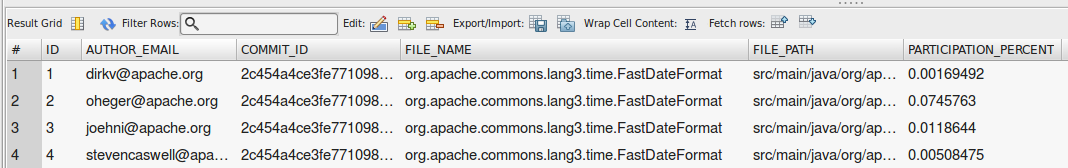
\includegraphics[width=1\textwidth]{img/case_study/participation.png}
	\caption{نمایی از جدول مشارکت‌کنندگان در ویرایش پرونده‌ها}
	\label{fig:participation}
\end{figure}


\begin{latin}
	\begin{lstlisting}[language=SQL]
SELECT max(PARTICIPATION_PERCENT) from Participation P 
where COMMIT_ID = :commitId AND FILE_NAME = :fileName")
\end{lstlisting}
\end{latin}
\captionof{lstlisting}{محاسبه‌ی درصد خطوط مالک پرونده}
\label{code:own}

\textbf{تعداد مشارکت‌کنندگان جزئی:‬}
 با استفاده از جدول Participation و پرسمان  \ref{code:minor}  معیار محاسبه می‌شود. مقدار minorThereshold برابر ۵ درصد قرار می‌گیرد.

\begin{latin}
	\begin{lstlisting}[language=SQL]
SELECT count(AUTHOR_EMAIL) from Participation P 
where COMMIT_ID = :commitId AND FILE_NAME = :fileName
and PARTICIPATION_PERCENT < :minorThreshold
\end{lstlisting}
\end{latin}
\captionof{lstlisting}{محاسبه‌ی تعداد مشارکت‌کنندگان جزئی}
\label{code:minor}

\textbf{تعداد ثبت‌های همسایگان:‬}
ابتدا لازم است که همسایگان پرونده در یک ثبت و نیز تعداد دفعات همسایگی در طول انتشار مشخص شود. این عمل به وسیله‌ی پرسمان \ref{code:neighbor} انجام می‌شود. سپس معیار تعداد ثبت‌ها در سیستم کنترل نسخه مشابه قبل با استفاده از کد \ref{code:comm} محاسبه می‌گردد و از آنها میانگین وزن‌دهی شده گرفته می‌شود.

\begin{latin}
\begin{lstlisting}[language=SQL]
SELECT FILE_NAME as `name`, count(ID) as `frequency` FROM
CommitChangedFile WHERE COMMIT_INFO_ID IN
	(SELECT COMMIT_INFO_ID FROM CommitChangedFile WHERE FILE_NAME = :fileName) 
AND COMMIT_INFO_ID IN
	(SELECT CI.ID from CommitInfo CI WHERE CI.SEQUENCE_NUMBER BETWEEN :startSeq AND :endSeq AND PROJECT = :project)
AND FILE_NAME != :fileName GROUP BY FILE_NAME
\end{lstlisting}
\end{latin}
\captionof{lstlisting}{یافتن همسایگان و تعدد همسایگی}
\label{code:neighbor}

\textbf{تعداد توسعه‌دهندگان فعال همسایگان:‬}
 به طور مشابه با معیار قبلی محاسبه می‌شود.\\
\textbf{‫تعداد توسعه‌دهندگان متمایز همسایگان:‬}
 به طور مشابه با معیار قبلی محاسبه می‌شود. \\

\textbf{تجربه‌ی مالک فایل:‬‬}
 برای محاسبه‌ی معیار ابتدا   با استفاده از پرسمان \ref{code:find-owner} مالک پرونده مشخص می‌شود. سپس تعداد ثبت‌هایی که مالک پرونده از ابتدای پروژه تا آن زمان ثبت کرده است  با استفاده از پرسمان \ref{code:commit-of-commiter} شمرده می‌شود. به ترتیب از دو جدول Participation 
 و 
 CommitInfo  استفاده می‌شود.

\begin{latin}
\begin{lstlisting}[language=SQL]
SELECT AUTHOR_EMAIL FROM Participation P WHERE COMMIT_ID = :commitId 
AND FILE_NAME = :fileName AND PARTICIPATION_PERCENT  = 
	(SELECT max(PARTICIPATION_PERCENT) FROM Participation P2 
	 WHERE P2.COMMIT_ID = :commitId  AND P2.FILE_NAME = :fileName)
\end{lstlisting}
\end{latin}
\captionof{lstlisting}{یافتن مالک پرونده}
\label{code:find-owner}



\begin{latin}
\begin{lstlisting}[language=SQL]
SELECT  count(*) from CommitInfo CI where CI.SEQUENCE_NUMBER BETWEEN
:startSeq AND :endSeq AND CI.PROJECT = :project AND CI.COMMITTER_MAIL =
:authorEmail
\end{lstlisting}
\end{latin}
\captionof{lstlisting}{شمارش تعداد ثبت‌های یک ثبت کننده در بازه‌ی زمانی داده شده}
\label{code:commit-of-commiter}

\textbf{‫تجربه‌ی تمام مشارکت‌کنندگان:‬}
ابتدا همه‌ی توسعه‌دهندگان پرونده با استفاده از پرسمان \ref{code:contributers} مشخص می‌شوند.  سپس میزان تجربه‌ی هر یک با استفاده از پرسمان \ref{code:commit-of-commiter} جداگانه محاسبه می‌شود و از آن‌ها میانگین هندسی گرفته می شود. 
\begin{latin}
\begin{lstlisting}[language=SQL]
SELECT AUTHOR_EMAIL FROM Participation P WHERE COMMIT_ID = :commitId 
AND FILE_NAME = :fileName
\end{lstlisting}
\end{latin}
\captionof{lstlisting}{یافتن مشارکت‌کنندگان در پرونده}
\label{code:contributers}


در نهایت جدولی برای معیارهای فرآیند تولید می‌شود که نمایی از آن در شکل \ref{fig:process-metics} آورده شده است. 
\begin{figure}[H]
	\centering
	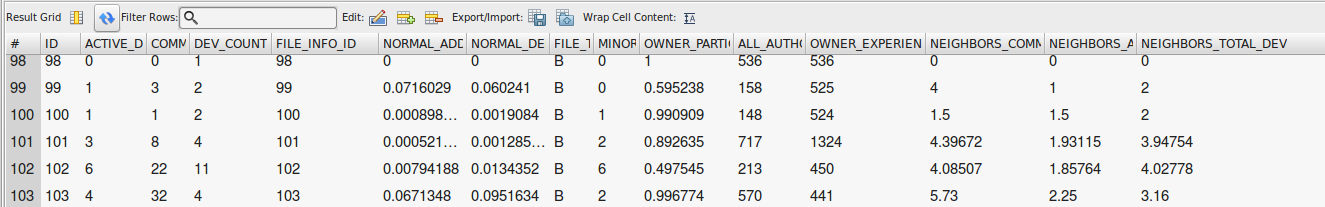
\includegraphics[width=1\textwidth]{img/case_study/process-metrics.png}
	\caption{نمایی از جدول معیارهای فرآیند }
	\label{fig:process-metics}
\end{figure}


\subsection{استخراج معیارهای جهش}
روند کلی به این صورت است که برای هر سطر از جدول BugInfo   یا CleanInfo که معادل یک  پرونده  در یک نسخه است ابتدا آن نسخه از برنامه در پوشه‌ی کاری قرار می‌گیرد. منظور از پوشه‌ی کاری محلی است  که پرونده‌های پروژه از مخزن نرم‌افزاری فراخوانی می‌شود و در آن قرار می گیرد. سپس به فایل build.xml    و یا build.gradle  قطعه کدهایی  به منظور  اجرای  صحیح فرآیند ساخت اضافه می‌شود.  \\
همچنین جهت تولید جهش‌یافته و تحلیل جهش لازم است برای هر پروژه پیکربندی‌هایی انجام شود که این پیکربندی‌ها با اجرای عملیات مهندسی معکوس در ابزار \lr{Defects4j} به دست آمد. به منظور انجام مهندسی معکوس کدهای ابزار که به زبان \نام{پرل}{Perl} نوشته شده‌اند مورد بررسی قرار گرفتند و نحوه‌ی عملکرد ابزار با پروژه‌های مختلف و پیکربندی‌ها مشخص شد. \\
از آنجا که اجرای تحلیل جهش زمان زیادی می‌گیرد برای انجام آن یک رایانه به صورت اختصاصی برای انجام آن در \نام{ آزمایشگاه کیفیت نرم‌افزار}{Software Quality Research Lab - \url{http://sqrlab.ce.sharif.edu/}} واقع در دانشگاه صنعتی شریف در نظر گرفته شد. این رایانه به یک سرور \نام{لینوکس}{Linux} تبدیل شد تا امکان نظارت و رفع خطا در استخراج معیارهای جهش همواره امکان پذیر باشد و استخراج معیارها و توسعه‌ی سایر قسمت‌های این پژوهش به صورت موازی انجام گیرد. جزییات تبدیل رایانه به سرور لینوکس در پیوست آمده است. \\
از آنجا که انجام تحلیل جهش بر روی موارد مطالعاتی صنعتی انجام گرفته است و پروژه‌های انتخاب شده حجم زیادی دارند لازم است تا پیکربندی‌هایی در نظر گرفته شود تا از بروز خطا و توقف محاسبات جلوگیری شود. این پیکربندی‌ها در زیر آمده است.  
\begin{itemize}
	 \setlength{\itemsep}{1pt}
	\setlength{\parskip}{0pt}
	\setlength{\parsep}{0pt}

\item 
\متن‌سیاه{افزایش فضای \نام{PermGen}{Premanent Generation}:}  
این فضا  یک \نام{هیپ}{Heap} مخصوص است که از فضای هیپ اصلی جاوا مجزا است و در آن \واژه{ماشین مجازی جاوا} \واژه[فراداده‌های]{فراداده} کلاس‌های بارگذاری شده را ردگیری می‌کند. به دلیل حجم زیاد پروژه‌های مورد مطالعه لازم است که این فضا بیشتر از حالت پیش‌فرض قرار داده شود. برای انجام این پژوهش فضای ۲ گیگابایت در نظر گرفته شده است. 
\item
\متن‌سیاه{افزایش فضای Codecache :} 
کدهای ترجمه شده به زبان ماشین در این فضا قرار می‌گیرد که به دلیل مشابه پیکربندی قبلی لازم است این فضا از حالت پیش‌فرض بیشتر باشد. فضای در نظر گرفته شده ۵۱۲ مگابایت می‌باشد. 
\item
\متن‌سیاه{قرار دادن \واژه{زمان خروج} :}
زمانی که یک جهش یافته از کد اصلی ساخته می‌شود ممکن است که جریان کنترلی به نحوی تغییر کند که برنامه در حلقه‌ی بی‌نهایت یا بن‌بست قرار گیرد. برای جلوگیری از چنین حالتی لازم است تا در تنظیمات ابزار JUnit  مهلت زمانی در نظر گرفته شود تا در صورت قرارگیری در چنین شرایطی پس از مدت زمان معین اجرای مورد آزمون متوقف شود و مورد آزمون شکست خورده تلقی شود. مدت زمان تعیین شده جهت خروج ۱۳ ثانیه می‌باشد. 
\متن‌سیاه{عملگرهای جهش انتخابی}
با توجه به هزینه‌ی زمانی تحلیل جهش به کارگیری تمامی عملگرهای موجود در ابزار Major به صرفه نمی‌باشد. برای تولید جهش‌یافته‌ها از مجموعه عملگرهای استفاده شده در مقاله‌ی بوئز و همکاران\cite{bowes2016mutation} استفاده شده که مطابق عملگرهای پیش‌فرض در ابزار   PIT‌ می‌باشد. پرونده‌ی MML ساخته شده در شکل \ref{fig:mml-used}

\begin{figure}[H]
	\centering
	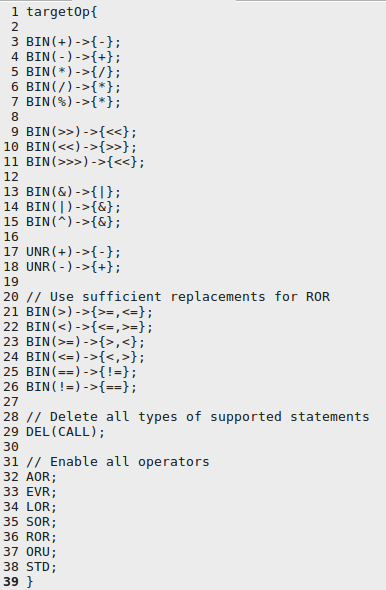
\includegraphics[width=.7\textwidth]{img/case_study/mml-used.png}
	\caption{پرونده‌ی mml ساخته شده جهت تولید جهش‌یافته‌ها}
	\label{fig:mml-used}
\end{figure}
\end{itemize}
 پس از انجام تحلیل جهش برای پرونده‌های حاوی خطا و سالم نتایج در جدول MutationMetrics قرار داده شد که نمایی از این جدول در شکل \ref{fig:mutation-metrics}  آمده است. 
 
 
 \begin{figure}[H]
 	\centering
 	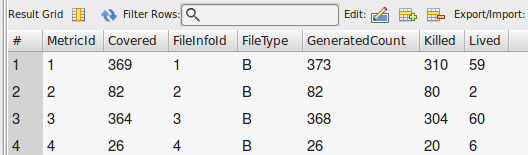
\includegraphics[width=.7\textwidth]{img/case_study/mutation-metrics.png}
 	\caption{نمایی از جدول نتایج تحلیل جهش}
 	\label{fig:mutation-metrics}
 \end{figure}
 
\subsection{ معیارهای فرآیند مبتنی بر جهش}
همانطور که در قسمت \ref{sec:method-phase-two} اشاره شده چهار معیار معرفی شدند و مبتنی بر جهش نامیده شدند. این قسمت به نحوه‌ی پیاده‌سازی دسته‌ی دوم از معیارها را شرح خواهد داد. 
\begin{itemize}
\item
\متن‌سیاه{تعداد جهش‌یافته‌های تولید شده‌ی جدید نسبت به انتشار قبلی برنامه:}
به منظور محاسبه‌ی این معیار ابتدا لازم است که مشخص شود که پرونده‌ی مورد نظر نسبت به انتشار قبلی چه تغییراتی داشته است. این کار با استفاده از ابزار JGit انجام  می‌شود. JGit این امکان را فراهم می‌کند که دو پرونده در دو ثبت متفاوت مقایسه شوند و مشخص می‌کند که کدام خطوط حذف شده‌اند و کدام خطوط اضافه شده‌اند. در اینجا لازم است خطوط اضافه شده  مشخص شود. سپس با استفاده از ابزار Major جهش‌یافته‌ها تولید می‌شود. در  قسمت  \ref{sec:tools-major} توضیح داده شد که پس تولید جهش‌یافته‌ها یک فایل خروجی نیز به نام mutant.log تولید می‌شود که در آن مشخص شده در هر خط از برنامه چه جهش‌یافته‌هایی تولید شده است. حال کافیست تعداد جهش‌یافته‌های تولید شده در خطوطی شمرده شوند که ابزار Jgit آن‌ها را به عنوان خطوط جدید نسبت به انتشار قبلی معرفی کرده است. بدین ترتیب این معیار محاسبه خواهد شد.\\
لازم به ذکر است روش یاد شده پایه‌ی محاسبه‌ی معیار بعدی و معیارهای رویکرد سوم است.
\item
\متن‌سیاه{تعداد جهش‌یافته‌های متمایز در چند انتشار اخیر:}

 به منظور افزایش کارایی ابتدا بررسی می‌شود که فایل مورد نظر در آن انتشار وجود دارد یا خیر در صورت عدم وجود محاسبات برای آن انتشار انجام نمی‌گیرد.
برای محاسبه ابتدا چهار انتشار قبلی  با استفاده از پرسمان  پرسمان مناسب از جدول ProjectRelease بازیابی می‌شود. سپس مشابه معیار قبلی جهش‌یافته‌های جدید نسبت به انتشار قبلی برای هر انتشار محاسبه می‌شود و با هم جمع زده می‌شود.  یک جدول برای نتایج تولید جهش‌یافته‌ها  به نام  DistinctMutantLog در نظر گرفته شده که تعداد جهش‌یافته‌های جدید برای هر انتشار نسبت به انتشار قبلی در آن ذخیره می‌گردد. از مزایای ایجاد این جدول پایداری در انجام محاسبات است به عنوان مثال  در صورت توقف محاسبات امکان از سرگیری محاسبات از محل توقف وجود  دارد و همچنین  با نگهداری به عنوان یک مجموعه داده می‌تواند در پژوهش‌های دیگر به کار گرفته شود. نمایی از جدول در شکل زیر آمده است. به طور مثال سطر اول جدول بیان می‌کند که در انتشاری از برنامه با شماره ثبت  \lr{..21a}  پرونده‌ی شماره یک شماره یک از فایلهای حاوی خطا 430 جهش‌یافته‌ی جدید نسبت به انتشار قبلی داشته است.
\begin{comment}
\begin{latin}
	\begin{lstlisting}[language=SQL]
SELECT * FROM ProjectRelease WHERE Project = :project AND
 SequenceNumber <  
	(SELECT SequenceNumber FROM ProjectRelease WHERE 
	 Project = :project AND CommitId = :releaseCommit) 
 ORDER BY SequenceNumber DESC LIMIT 4 
\end{lstlisting}
\end{latin}
\captionof{lstlisting}{بازیابی چهار نسخه‌ی اخیر یک ثبت}
\label{code:previous-releases}
\end{comment}

\begin{figure}[H]
	\centering
	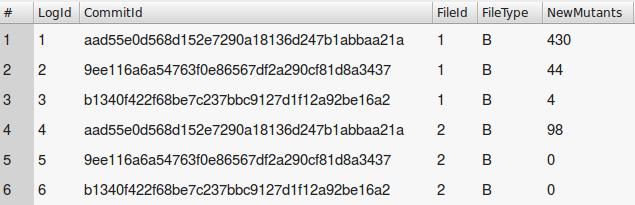
\includegraphics[width=1\textwidth]{img/case_study/distinct-mutant-log.png}
	\caption{نمایی از جدول تعداد جهش‌یافته‌های متمایز در انتشارها}
	\label{fig:distinct-mutant-log}
\end{figure}
\item
\متن‌سیاه{میزان تغییرات مثبت امتیاز جهش  در چند انتشار اخیر:}
ابتدا انتشارها  مشابه معیار قبلی بازیابی می‌شوند و سپس برای هر یک تحلیل جهش انجام می‌گردد. نتایج جهش در جدولی به نام ReleaseMutation قرار می‌گیرد.  نمایی از این جدول در شکل  \ref{fig:release-mutation} آمده است. سپس هر انتشار با انتشار قبلی مقایسه می‌شود و در صورتی که تغییر امتیاز جهش  مثبت باشد با مجموعه تغییرات مثبت جمع می‌گردد. 
\begin{figure}[H]
	\centering
	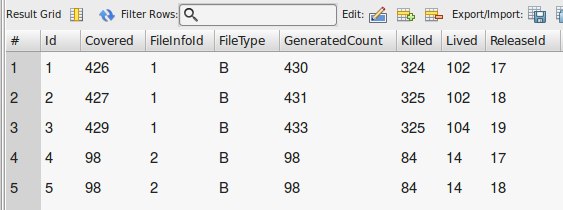
\includegraphics[width=1\textwidth]{img/case_study/release-mutation.png}
	\caption{نمایی از جدول نتایج تحلیل جهش در انتشارها}
	\label{fig:release-mutation}
\end{figure}
\item
\متن‌سیاه{میزان تغییرات منفی امتیاز جهش  در چند انتشار اخیر:}
به طور مشابه با معیار قبلی عمل می‌گردد با این تفاوت که تغییرات منفی در نظر گرفته می‌شود. 
\end{itemize}

\subsection{معیارهای ترکیبی جهش-فرآیند}

نحوه‌ی محاسبه به این صورت خواهید بود که ابتدا ثبت‌هایی از برنامه در طول آخرین انتشار که در آن فایل مورد نظر تغییر کرده است  توسط  پرسمان   مناسب بازیابی می شود. سپس برای هر ثبت تعداد جهش یافته‌های جدید نسبت به ثبت قبلی محاسبه می‌شود و برای محاسبه‌ی جهش‌یافته‌های حذف شده تعداد جهش یافته‌ها در  ثبت قبلی را یافته و آن‌ها که جز خطوط حذف شده در ثبت بعدی است شمرده می شود. تعداد جهش‌یافته‌های اضافه و حذف شده در ثبت‌ها جمع شده و بر تعداد ثبت‌های کل پروژه در طول انتشار تقسیم می گردد.

\begin{comment}

\begin{latin}
\begin{lstlisting}[language=SQL]
SELECT CC.* from CommitChangedFile CC, CommitInfo CI where CC.COMMIT_INFO_ID = CI.ID
AND CI.SEQUENCE_NUMBER BETWEEN :startSeq AND :endSeq
AND CI.PROJECT = :project
AND CC.FILE_NAME = :fileName ORDER BY CI.SEQUENCE_NUMBER asc
\end{lstlisting}
\end{latin}
\captionof{lstlisting}{بازیابی اطلاعات ثبت‌هایی که یک فایل در بازه‌ی مشخص در آنها تغییر کرده است}
\label{code:commit-during-release}
\end{comment}